% Options for packages loaded elsewhere
% Options for packages loaded elsewhere
\PassOptionsToPackage{unicode}{hyperref}
\PassOptionsToPackage{hyphens}{url}
\PassOptionsToPackage{dvipsnames,svgnames,x11names}{xcolor}
%
\documentclass[
  11pt,
  a4paper,
]{article}
\usepackage{xcolor}
\usepackage[margin=1in]{geometry}
\usepackage{amsmath,amssymb}
\setcounter{secnumdepth}{5}
\usepackage{iftex}
\ifPDFTeX
  \usepackage[T1]{fontenc}
  \usepackage[utf8]{inputenc}
  \usepackage{textcomp} % provide euro and other symbols
\else % if luatex or xetex
  \usepackage{unicode-math} % this also loads fontspec
  \defaultfontfeatures{Scale=MatchLowercase}
  \defaultfontfeatures[\rmfamily]{Ligatures=TeX,Scale=1}
\fi
\usepackage{lmodern}
\ifPDFTeX\else
  % xetex/luatex font selection
\fi
% Use upquote if available, for straight quotes in verbatim environments
\IfFileExists{upquote.sty}{\usepackage{upquote}}{}
\IfFileExists{microtype.sty}{% use microtype if available
  \usepackage[]{microtype}
  \UseMicrotypeSet[protrusion]{basicmath} % disable protrusion for tt fonts
}{}
\makeatletter
\@ifundefined{KOMAClassName}{% if non-KOMA class
  \IfFileExists{parskip.sty}{%
    \usepackage{parskip}
  }{% else
    \setlength{\parindent}{0pt}
    \setlength{\parskip}{6pt plus 2pt minus 1pt}}
}{% if KOMA class
  \KOMAoptions{parskip=half}}
\makeatother
% Make \paragraph and \subparagraph free-standing
\makeatletter
\ifx\paragraph\undefined\else
  \let\oldparagraph\paragraph
  \renewcommand{\paragraph}{
    \@ifstar
      \xxxParagraphStar
      \xxxParagraphNoStar
  }
  \newcommand{\xxxParagraphStar}[1]{\oldparagraph*{#1}\mbox{}}
  \newcommand{\xxxParagraphNoStar}[1]{\oldparagraph{#1}\mbox{}}
\fi
\ifx\subparagraph\undefined\else
  \let\oldsubparagraph\subparagraph
  \renewcommand{\subparagraph}{
    \@ifstar
      \xxxSubParagraphStar
      \xxxSubParagraphNoStar
  }
  \newcommand{\xxxSubParagraphStar}[1]{\oldsubparagraph*{#1}\mbox{}}
  \newcommand{\xxxSubParagraphNoStar}[1]{\oldsubparagraph{#1}\mbox{}}
\fi
\makeatother


\usepackage{longtable,booktabs,array}
\usepackage{calc} % for calculating minipage widths
% Correct order of tables after \paragraph or \subparagraph
\usepackage{etoolbox}
\makeatletter
\patchcmd\longtable{\par}{\if@noskipsec\mbox{}\fi\par}{}{}
\makeatother
% Allow footnotes in longtable head/foot
\IfFileExists{footnotehyper.sty}{\usepackage{footnotehyper}}{\usepackage{footnote}}
\makesavenoteenv{longtable}
\usepackage{graphicx}
\makeatletter
\newsavebox\pandoc@box
\newcommand*\pandocbounded[1]{% scales image to fit in text height/width
  \sbox\pandoc@box{#1}%
  \Gscale@div\@tempa{\textheight}{\dimexpr\ht\pandoc@box+\dp\pandoc@box\relax}%
  \Gscale@div\@tempb{\linewidth}{\wd\pandoc@box}%
  \ifdim\@tempb\p@<\@tempa\p@\let\@tempa\@tempb\fi% select the smaller of both
  \ifdim\@tempa\p@<\p@\scalebox{\@tempa}{\usebox\pandoc@box}%
  \else\usebox{\pandoc@box}%
  \fi%
}
% Set default figure placement to htbp
\def\fps@figure{htbp}
\makeatother


% definitions for citeproc citations
\NewDocumentCommand\citeproctext{}{}
\NewDocumentCommand\citeproc{mm}{%
  \begingroup\def\citeproctext{#2}\cite{#1}\endgroup}
\makeatletter
 % allow citations to break across lines
 \let\@cite@ofmt\@firstofone
 % avoid brackets around text for \cite:
 \def\@biblabel#1{}
 \def\@cite#1#2{{#1\if@tempswa , #2\fi}}
\makeatother
\newlength{\cslhangindent}
\setlength{\cslhangindent}{1.5em}
\newlength{\csllabelwidth}
\setlength{\csllabelwidth}{3em}
\newenvironment{CSLReferences}[2] % #1 hanging-indent, #2 entry-spacing
 {\begin{list}{}{%
  \setlength{\itemindent}{0pt}
  \setlength{\leftmargin}{0pt}
  \setlength{\parsep}{0pt}
  % turn on hanging indent if param 1 is 1
  \ifodd #1
   \setlength{\leftmargin}{\cslhangindent}
   \setlength{\itemindent}{-1\cslhangindent}
  \fi
  % set entry spacing
  \setlength{\itemsep}{#2\baselineskip}}}
 {\end{list}}
\usepackage{calc}
\newcommand{\CSLBlock}[1]{\hfill\break\parbox[t]{\linewidth}{\strut\ignorespaces#1\strut}}
\newcommand{\CSLLeftMargin}[1]{\parbox[t]{\csllabelwidth}{\strut#1\strut}}
\newcommand{\CSLRightInline}[1]{\parbox[t]{\linewidth - \csllabelwidth}{\strut#1\strut}}
\newcommand{\CSLIndent}[1]{\hspace{\cslhangindent}#1}



\setlength{\emergencystretch}{3em} % prevent overfull lines

\providecommand{\tightlist}{%
  \setlength{\itemsep}{0pt}\setlength{\parskip}{0pt}}



 


\makeatletter
\@ifpackageloaded{caption}{}{\usepackage{caption}}
\AtBeginDocument{%
\ifdefined\contentsname
  \renewcommand*\contentsname{Table of contents}
\else
  \newcommand\contentsname{Table of contents}
\fi
\ifdefined\listfigurename
  \renewcommand*\listfigurename{List of Figures}
\else
  \newcommand\listfigurename{List of Figures}
\fi
\ifdefined\listtablename
  \renewcommand*\listtablename{List of Tables}
\else
  \newcommand\listtablename{List of Tables}
\fi
\ifdefined\figurename
  \renewcommand*\figurename{Figure}
\else
  \newcommand\figurename{Figure}
\fi
\ifdefined\tablename
  \renewcommand*\tablename{Table}
\else
  \newcommand\tablename{Table}
\fi
}
\@ifpackageloaded{float}{}{\usepackage{float}}
\floatstyle{ruled}
\@ifundefined{c@chapter}{\newfloat{codelisting}{h}{lop}}{\newfloat{codelisting}{h}{lop}[chapter]}
\floatname{codelisting}{Listing}
\newcommand*\listoflistings{\listof{codelisting}{List of Listings}}
\makeatother
\makeatletter
\makeatother
\makeatletter
\@ifpackageloaded{caption}{}{\usepackage{caption}}
\@ifpackageloaded{subcaption}{}{\usepackage{subcaption}}
\makeatother
\usepackage{bookmark}
\IfFileExists{xurl.sty}{\usepackage{xurl}}{} % add URL line breaks if available
\urlstyle{same}
\hypersetup{
  pdftitle={Multi-modal LLM for Financial Decision Intelligence: Integrating News Text and Stock Price Time-Series via Cross-Modal Attention},
  pdfauthor={Cooperation.TW},
  pdfkeywords={Multi-modal learning, Large language models, Financial
decision intelligence, Cross-modal attention, Asset pricing, Information
asymmetry},
  colorlinks=true,
  linkcolor={blue},
  filecolor={Maroon},
  citecolor={blue},
  urlcolor={blue},
  pdfcreator={LaTeX via pandoc}}


\title{Multi-modal LLM for Financial Decision Intelligence: Integrating
News Text and Stock Price Time-Series via Cross-Modal Attention}
\author{Cooperation.TW}
\date{2026-03-20}
\begin{document}
\maketitle
\begin{abstract}
Financial return prediction systems have traditionally been constrained
to single-modality inputs --- either textual sentiment or historical
price dynamics --- despite the complementary nature of these information
channels. Existing multi-modal finance models lack both a theoretically
grounded fusion mechanism and rigorous econometric identification of the
incremental information content contributed by each modality. This paper
introduces FinMM-LLM, a multi-modal large language model that integrates
financial news text and stock price time-series through a bidirectional
cross-modal attention architecture. News articles are encoded via a
domain-adapted FinBERT encoder, price histories are represented as
patch-level tokens using a PatchTST backbone, and a gated
cross-attention layer learns to dynamically weight each modality's
contribution to the joint representation. The model is evaluated on a
survivorship-bias-free panel of S\&P 500 constituents over the
2018--2024 period, using approximately 500,000 financial news articles
matched to daily OHLCV data. The multi-modal strategy achieves an
out-of-sample annualized Sharpe ratio of 1.55\textsuperscript{S},
compared with 1.10\textsuperscript{S} for the time-series-only baseline
and 0.85\textsuperscript{S} for the text-only baseline, representing a
41\% relative improvement. A Fama-French five-factor alpha of
72\textsuperscript{S} basis points per month (t =
3.41\textsuperscript{S}) confirms that the excess returns are not
attributable to standard risk exposures. Conditional analysis reveals
that alpha is particularly concentrated around earnings announcements
(118\textsuperscript{S} bps versus 68\textsuperscript{S} bps in
non-announcement windows), and that the cross-modal attention intensity
is positively correlated with the VIX (ρ = 0.64\textsuperscript{S}).
Attention decomposition identifies a gradual information diffusion
mechanism consistent with Hong and Stein
(\citeproc{ref-HongStein1999}{1999}), wherein textual signals contribute
incremental predictive content over price paths in high-information
regimes where markets have not yet achieved full price discovery. These
results suggest that multi-modal fusion architectures are most valuable
not as general performance enhancers, but as targeted instruments for
capturing regime-conditional information asymmetries.

\textsuperscript{S} = simulated value (MVP mode). All numerical results
are statistically self-consistent simulations pending real data
collection.
\end{abstract}


\section{Introduction}\label{introduction}

Financial markets are shaped by the continuous flow of information
across heterogeneous channels. At the most fundamental level, two
complementary streams govern price discovery: textual
information---encompassing news articles, earnings call transcripts, and
regulatory filings---and quantitative time-series data, including
prices, volumes, and technical indicators. The pioneering work of
Tetlock (\citeproc{ref-Tetlock2007}{2007}) demonstrated that the
pessimism embedded in financial media exerts measurable downward
pressure on equity prices, while Da et al. (\citeproc{ref-Da2011}{2011})
showed that investor attention, proxied by internet search volume,
predicts short-horizon return reversals consistent with sentiment-driven
demand. At the same time, the empirical asset pricing literature,
exemplified by Gu et al. (\citeproc{ref-Gu2020}{2020}), has documented
that machine learning methods applied to structured market data yield
economically large risk premia. The recent revolution in large language
models (LLMs), surveyed by Gentzkow et al.
(\citeproc{ref-Gentzkow2019}{2019}) as part of the broader ``text as
data'' paradigm, has further opened the possibility of processing
financial discourse at unprecedented scale and semantic depth. Yet
despite the clear complementarity between these two information
channels, the overwhelming majority of existing models treat them
independently---leaving substantial predictive information and economic
insight on the table.

Three fundamental gaps characterize the current state of the literature.
First, text-based and time-series-based approaches have evolved along
largely parallel tracks with minimal integration. On the textual side,
Lopez-Lira and Tang (\citeproc{ref-LopezLiraTang2023}{2023}) and Chen et
al. (\citeproc{ref-ChenKellyXiu2023}{2023}) have demonstrated that
LLM-derived sentiment scores carry substantial cross-sectional
predictive power for stock returns; on the quantitative side, Nie et al.
(\citeproc{ref-Nie2023}{2023}) and Liu et al.
(\citeproc{ref-Liu2024}{2024}) have advanced the architecture of
Transformer-based forecasters for time-series data. However, these two
lines of inquiry are conducted in isolation, and the question of whether
text and price signals provide genuinely incremental information---or
merely replicate one another---remains unresolved. Second, the existing
LLM finance literature focuses predominantly on predictive accuracy
without grounding findings in economic mechanism. Studies such as Kirtac
and Germano (\citeproc{ref-KirtacGermano2024}{2024}) and Guo and
Hauptmann (\citeproc{ref-Guo2024}{2024}) report impressive return
forecasts but offer little insight into \emph{why} language models
capture return variation---whether through fundamental information,
investor attention, or liquidity dynamics. This absence of economic
identification limits the theoretical interpretation and practical
credibility of LLM-based trading strategies. Third, no existing
multi-modal framework systematically examines how the joint predictive
power of text and price data varies across market regimes. The work of
Zong et al. (\citeproc{ref-Zong2025}{2025}) and Zhang and Zhang
(\citeproc{ref-DeepFusion2024}{2024}) demonstrates the feasibility of
multi-modal fusion for stock prediction but does not condition on
volatility states or macroeconomic cycles, obscuring the circumstances
under which each modality dominates and leaving asset managers without
actionable guidance for regime-dependent allocation.

This paper introduces \textbf{FinMM-LLM}, a multi-modal large language
model architecture designed to address all three gaps simultaneously.
The contributions of this work are threefold. First, a novel cross-modal
attention architecture is proposed in which a language encoder and a
patch-based time-series encoder are aligned through a shared latent
space, with cross-attention heads that dynamically weight each modality
as a function of the input context. This architecture builds on the
general multi-modal learning framework of Baltrusaitis et al.
(\citeproc{ref-Baltrusaitis2019}{2019}) and extends it to the specific
demands of financial decision intelligence. Second, large-scale
empirical evidence is provided that textual and time-series signals
carry \emph{incremental} predictive information: using a comprehensive
sample of S\&P 500 constituents over seven years, the multi-modal
portfolio generates a statistically and economically significant alpha
against the Fama and French (\citeproc{ref-Fama2015}{2015}) five-factor
model, indicating that cross-modal integration is not subsumed by known
risk factors. Third, a cross-modal attention decomposition analysis is
performed to interpret the learned representations through the lens of
the information diffusion theory of Hong and Stein
(\citeproc{ref-HongStein1999}{1999}), showing that attention weights
assigned to the textual channel spike precisely in the windows
surrounding analyst revisions and earnings announcements---consistent
with the mechanism of gradual information diffusion posited by Glosten
and Milgrom (\citeproc{ref-GlostenMilgrom1985}{1985}). Together, these
contributions advance both the engineering frontier of multi-modal AI
and the economic understanding of how heterogeneous information is
priced in equity markets.

The remainder of this paper is organized as follows. The following
section surveys the related literature across three strands: financial
text mining, machine learning for asset pricing, and multi-modal
learning with time-series Transformers. The model architecture and
training procedure are then described (see Figure~\ref{fig-framework}
for an overview), followed by the data construction and empirical
design. Main predictive performance results are subsequently presented,
with portfolio-level and factor-model-based evaluation. The attention
decomposition analysis and regime-conditional tests are reported next.
The final section concludes and identifies directions for future
research.

\begin{figure}

\centering{


\includegraphics[width=1\linewidth,height=\textheight,keepaspectratio]{figures/fig1_framework.png}

}

\caption{\label{fig-framework}FinMM-LLM architecture. Financial news
text is encoded via FinBERT (left, blue), OHLCV price series via
PatchTST (right, orange). Bidirectional cross-modal attention (center,
purple) aligns the two modalities, and a gated fusion layer (green)
produces the final portfolio signal.}

\end{figure}%

\section{Related Work}\label{related-work}

\subsection{Financial Text Mining: From Dictionaries to Large Language
Models}\label{financial-text-mining-from-dictionaries-to-large-language-models}

The systematic extraction of information from financial text has a long
history in the empirical finance and NLP literatures. Early
dictionary-based approaches operationalized sentiment by counting words
drawn from curated lexicons. Tetlock (\citeproc{ref-Tetlock2007}{2007})
provided seminal evidence that the fraction of pessimistic language in
financial news columns predicts market returns and trading volume.
Tetlock et al. (\citeproc{ref-Tetlock2008}{2008}) extended this
framework to firm-level news and showed that the share of negative words
from general-purpose dictionaries forecasts accounting earnings and
stock returns, though their predictive power decays rapidly. A critical
methodological advance came from Loughran and McDonald
(\citeproc{ref-LoughranMcDonald2011}{2011}), who demonstrated that
Harvard's General Inquirer lexicon systematically misclassifies
financial terminology---labeling ``liability'' and ``tax'' as negative
despite their neutral connotations in financial discourse---and proposed
a finance-specific word list that substantially improves return
predictability in 10-K filings. The arrival of deep learning prompted a
fundamental rethinking of textual representation. Ding et al.
(\citeproc{ref-Ding2015}{2015}) proposed extracting structured events
from news and encoding them via a neural tensor network, demonstrating
that event-driven features carry incremental predictive content beyond
dictionary sentiment scores. Domain-adapted language models then emerged
as the dominant paradigm: Araci (\citeproc{ref-Araci2019}{2019})
fine-tuned BERT on a financial communication corpus to produce FinBERT,
and Yang et al. (\citeproc{ref-Yang2020}{2020}) scaled this approach to
4.9 billion tokens spanning corporate reports, earnings calls, and
analyst reports. The most recent wave has harnessed general-purpose
LLMs: Wu et al. (\citeproc{ref-Wu2023}{2023}) trained BloombergGPT on a
proprietary 363-billion-token financial archive, while Yang et al.
(\citeproc{ref-Yang2023}{2023}) introduced the open-source FinGPT
framework with reinforcement learning from human feedback. In the
cross-sectional return prediction domain, Lopez-Lira and Tang
(\citeproc{ref-LopezLiraTang2023}{2023}) documented that ChatGPT
sentiment scores derived from news headlines significantly predict
next-day abnormal returns, and Chen et al.
(\citeproc{ref-ChenKellyXiu2023}{2023}) showed that LLM-based signals
generate Sharpe-ratio improvements that are incremental to both
price-based and characteristic-based strategies. Guo and Hauptmann
(\citeproc{ref-Guo2024}{2024}) further investigated fine-tuning
strategies for return prediction from newsflow, comparing encoder-only
and decoder-only architectures. Despite this remarkable progress, a
common limitation of all text-based approaches is that textual signals
are processed in isolation, without joint modeling alongside the
quantitative price dynamics that evolve contemporaneously with news
flow.

\subsection{Machine Learning for Asset
Pricing}\label{machine-learning-for-asset-pricing}

The application of machine learning methods to the canonical asset
pricing problem---measuring and forecasting risk premia---was
systematically benchmarked by Gu et al. (\citeproc{ref-Gu2020}{2020}),
who documented that neural networks and gradient-boosted trees applied
to a large panel of firm characteristics nearly double the out-of-sample
Sharpe ratio relative to leading regression-based approaches. The
dimensionality reduction perspective was formalized by Kelly et al.
(\citeproc{ref-Kelly2019}{2019}), who showed that when factor loadings
are modeled as functions of observable characteristics, a unified
framework nests both factor models and characteristic-based pricing
models. The interface between textual information and cross-sectional
returns was examined by Ke et al. (\citeproc{ref-KeKellyXiu2019}{2019}),
who introduced a supervised text-mining method yielding sentiment scores
that predict individual stock returns and earnings surprises,
outperforming commercial sentiment vendors. Gentzkow et al.
(\citeproc{ref-Gentzkow2019}{2019}) provided the methodological
foundation for treating text as structured economic data, surveying a
broad class of approaches including bag-of-words, topic models, and word
embeddings. A distinct and visually oriented branch of the literature
was advanced by Jiang et al. (\citeproc{ref-Jiang2023}{2023}), who
applied convolutional neural networks to images of stock price charts
and demonstrated that chart-based signals generate significant
out-of-sample return predictability with gradient-based economic
interpretation. Despite these advances, the prevailing approach in the
machine learning asset pricing literature remains anchored to a single
modality---either quantitative characteristics, text, or visual price
representations---or, when multiple signals are combined, relies on
simple feature concatenation rather than principled cross-modal
alignment. This limitation restricts the capacity of existing models to
exploit the information complementarity that economic theory predicts
should exist between fundamental news and price dynamics.

\subsection{Multi-Modal Learning and Time-Series
Transformers}\label{multi-modal-learning-and-time-series-transformers}

The theoretical foundation for integrating heterogeneous information
streams is provided by the multi-modal machine learning framework of
Baltrusaitis et al. (\citeproc{ref-Baltrusaitis2019}{2019}), who
identified five core challenges in multi-modal systems---representation,
translation, alignment, fusion, and co-learning---and argued that joint
modeling consistently outperforms late fusion of unimodal systems. The
Transformer architecture introduced by Vaswani et al.
(\citeproc{ref-Vaswani2017}{2017}) has become the backbone of both
modalities considered in this paper: large language models derive their
text comprehension capabilities from scaled self-attention, and the
time-series domain has been reshaped by a succession of Transformer
variants. Zhou et al. (\citeproc{ref-Zhou2021}{2021}) proposed Informer
with ProbSparse self-attention for long-horizon forecasting; Wu et al.
(\citeproc{ref-Wu2021}{2021}) introduced Autoformer with
decomposition-based auto-correlation; Lim et al.
(\citeproc{ref-Lim2021}{2021}) developed the Temporal Fusion Transformer
for interpretable multi-horizon forecasting with explicit variable
selection; and patch-based representations were advanced by Nie et al.
(\citeproc{ref-Nie2023}{2023}), who showed that a time series is worth
64 words---treating subseries as tokens dramatically improves long-range
forecasting. Liu et al. (\citeproc{ref-Liu2024}{2024}) further refined
the Transformer's role in time-series modeling through inverted
attention across variate dimensions. The vision-language alignment
paradigm demonstrated by Radford et al.
(\citeproc{ref-Radford2021}{2021}) in CLIP established a blueprint for
grounding representations across fundamentally different signal types
via contrastive pre-training. The multi-modal financial prediction
literature has grown rapidly in response: Xu and Cohen
(\citeproc{ref-Xu2018}{2018}) proposed StockNet, a generative model that
jointly processes tweets and historical price movements; Zhang and Zhang
(\citeproc{ref-DeepFusion2024}{2024}) combined a fine-tuned BERT branch
with an LSTM-based price branch for stock prediction; Ye et al.
(\citeproc{ref-Ye2024}{2024}) fused historical prices with news
embeddings through an information-theoretic fusion objective; and Zong
et al. (\citeproc{ref-Zong2025}{2025}) introduced a gated
cross-attention mechanism that fuses indicator sequences, textual news,
and relational graphs, reporting 8--32\% improvements over unimodal
baselines. Despite this growing body of work, existing multi-modal
finance models share two critical limitations: they provide no economic
identification mechanism that would allow the learned representations to
be interpreted within established theories of information diffusion or
adverse selection, and they do not conduct regime-conditional analysis
that would reveal when and why each modality contributes to return
predictability. The present paper occupies the upper-right quadrant of a
two-dimensional space defined by (i) multi-modal integration versus
single-modality and (ii) economic interpretability versus black-box
prediction---a position currently unoccupied by any existing work---and
thus addresses both limitations simultaneously through cross-modal
attention decomposition and regime-stratified evaluation.

\section{Methodology}\label{methodology}

\subsection{Problem Formulation}\label{problem-formulation}

A formal prediction task is defined over a universe of stocks indexed by
\(i\), observed across trading days indexed by \(t\). For each stock-day
pair \((i, t)\), two input modalities are made available: a text corpus
\(\mathcal{T}_{i,t}\) comprising financial news articles published
within the trading day, and a historical price series
\(\mathbf{P}_{i,t-L:t} \in \mathbb{R}^{L \times 5}\) representing \(L\)
consecutive trading days of open, high, low, close, and volume (OHLCV)
observations. The objective is to predict the forward return
\(r_{i,t+h}\) at prediction horizons \(h \in \{1, 5, 20\}\) trading
days, corresponding respectively to daily, weekly, and monthly
investment signals.

The joint investment signal is formulated as

\[s_{i,t} = f\!\left(\mathcal{T}_{i,t},\, \mathbf{P}_{i,t-L:t};\, \theta\right),\]

where \(f(\cdot;\theta)\) denotes the proposed FinMM-LLM framework
parameterized by \(\theta\). Stocks are ranked by \(s_{i,t}\) at each
rebalancing date, and a long-short decile portfolio is constructed from
the top and bottom deciles. This formulation enables systematic
comparison across horizons and facilitates factor-adjusted evaluation
against standard asset pricing benchmarks.

\subsection{Text Encoder}\label{text-encoder}

Financial news text is encoded using FinBERT
(\citeproc{ref-Yang2020}{Yang et al., 2020}), a domain-adapted variant
of BERT (\citeproc{ref-Devlin2019}{Devlin et al., 2019}) pre-trained on
a large corpus of financial communication. For each stock-day pair, the
title and leading 512 tokens of each retrieved news article are supplied
as input, a truncation strategy that preserves the highest-density
information while remaining within the model's context window.

Let \(N_t\) denote the number of articles associated with stock \(i\) on
day \(t\). The encoder produces a set of article-level embeddings

\[\mathbf{e}^{(k)}_{i,t} \in \mathbb{R}^{d_t}, \quad k = 1, \ldots, N_t,\]

where \(d_t = 768\) is the hidden dimension of FinBERT. Because \(N_t\)
varies across stock-day pairs, a learnable attention pooling mechanism
is employed to aggregate the article set into a fixed-size
representation. Specifically, scalar attention weights \(\alpha^{(k)}\)
are computed via a single linear projection followed by a softmax
normalization, and the stock-day text representation is obtained as the
weighted sum
\(\mathbf{v}_{i,t} = \sum_{k} \alpha^{(k)} \mathbf{e}^{(k)}_{i,t}\). The
resulting matrix \(\mathbf{T}_{i,t} \in \mathbb{R}^{N_t \times d_t}\)
retains article-level granularity for subsequent cross-modal attention.

Two alternatives are examined in the ablation study: (i) embeddings
extracted from a general-purpose GPT encoder
(\citeproc{ref-Brown2020}{Brown et al., 2020}), and (ii) document-level
sentiment scores derived from the Loughran-McDonald financial lexicon
(\citeproc{ref-LoughranMcDonald2011}{Loughran and McDonald, 2011}),
which provides a non-parametric baseline. FinBERT is selected as the
primary encoder owing to its superior in-domain calibration and its
demonstrated advantage in financial sentiment classification tasks.

\subsection{Time-Series Encoder}\label{time-series-encoder}

Historical price dynamics are encoded using the PatchTST architecture
(\citeproc{ref-Nie2023}{Nie et al., 2023}), a transformer-based
time-series model that processes multivariate sequences through
non-overlapping temporal patches. The OHLCV price series
\(\mathbf{P}_{i,t-L:t} \in \mathbb{R}^{L \times 5}\) is constructed with
a lookback window of \(L = 60\) trading days, approximately three
calendar months of observations.

Each variate channel is divided into non-overlapping patches of length
\(P = 5\) days, yielding \(N_s = \lfloor L / P \rfloor = 12\) patch
tokens per channel. A channel-independent projection maps each patch to
a \(d_s = 128\)-dimensional embedding, producing a patch token sequence
\(\mathbf{S}_{i,t} \in \mathbb{R}^{N_s \times d_s}\). Sinusoidal
positional encodings are added to \(\mathbf{S}_{i,t}\) to preserve
temporal ordering across patches, a property that is critical for
capturing trend and momentum signals.

The patch-based design was chosen over token-per-timestep alternatives
because it reduces sequence length by a factor of \(P\), mitigating the
quadratic cost of self-attention while capturing local temporal
structure within each patch. Two alternatives are included in the
ablation: a bidirectional LSTM (\citeproc{ref-Hochreiter1997}{Hochreiter
and Schmidhuber, 1997}) that processes the flattened OHLCV sequence
recurrently, and iTransformer (\citeproc{ref-Liu2024}{Liu et al.,
2024}), a recently proposed variant that applies attention across
variate dimensions rather than the time dimension. PatchTST is selected
as the primary backbone based on preliminary validation performance and
its established superiority on multi-step financial forecasting
benchmarks.

\subsection{Cross-Modal Attention Fusion}\label{sec-fusion}

The cross-modal fusion module constitutes the central methodological
contribution of FinMM-LLM. Rather than combining text and price
representations through simple concatenation or element-wise operations,
a bidirectional cross-attention mechanism is introduced to enable each
modality to selectively query information from the other. This design is
motivated by the observation that the informativeness of price movements
is often contingent on the sentiment context provided by contemporaneous
news, and vice versa.

Formally, let \(\mathbf{T} \in \mathbb{R}^{N_t \times d_t}\) and
\(\mathbf{S} \in \mathbb{R}^{N_s \times d_s}\) denote the text and price
token sequences, respectively, projected to a common dimension \(d_k\)
via learned linear maps \(W_Q, W_K, W_V\). The text-to-price
cross-attention is defined as

\[\mathrm{CrossAttn}(\mathbf{T}, \mathbf{S}) = \mathrm{softmax}\!\left(\frac{\mathbf{T} W_Q \left(\mathbf{S} W_K\right)^\top}{\sqrt{d_k}}\right) \mathbf{S} W_V,\]

where \(\mathbf{T}\) serves as the query source and \(\mathbf{S}\)
provides keys and values. An analogous price-to-text operation is
computed symmetrically, with roles reversed. The resulting
cross-attended representations from both directions are concatenated and
passed through a layer normalization.

A gated fusion layer then combines the cross-modal output \(\mathbf{C}\)
with the original price representation via a data-dependent gate:

\[\mathbf{F} = \sigma(W_g \mathbf{C}) \odot \mathbf{C} + \left(1 - \sigma(W_g \mathbf{C})\right) \odot \mathbf{S},\]

where \(\sigma(\cdot)\) is the sigmoid function and \(\odot\) denotes
element-wise multiplication. This formulation allows the model to
adaptively suppress the cross-modal component when text signals are
uninformative, reverting to a near-unimodal price representation.

The architecture draws conceptual inspiration from CLIP-style
contrastive alignment (\citeproc{ref-Radford2021}{Radford et al., 2021})
but is substantially adapted for sequential, heterogeneous financial
data in which the two modalities differ in sequence length, token
semantics, and temporal granularity. Connections to the broader
multi-modal learning literature are discussed in Baltrusaitis et al.
(\citeproc{ref-Baltrusaitis2019}{2019}), while the foundational
self-attention mechanism follows Vaswani et al.
(\citeproc{ref-Vaswani2017}{2017}). An important interpretability
benefit of the cross-attention design is that the attention weight
matrix \(\boldsymbol{\alpha} \in \mathbb{R}^{N_t \times N_s}\) can be
inspected post-hoc to identify which text tokens most strongly activate
which price patches, providing a granular view of cross-modal
interaction that is exploited in the conditional analysis
(\citeproc{ref-Zong2025}{Zong et al., 2025}).

\subsection{Evaluation Framework}\label{evaluation-framework}

A long-short decile portfolio strategy is employed as the primary
evaluation vehicle. At each rebalancing date, stocks are sorted by the
predicted signal \(s_{i,t}\) and assigned to ten equal-weight deciles;
the portfolio goes long on the top decile and short on the bottom
decile, with daily rebalancing. Performance is summarized through four
metrics: annualized Sharpe ratio, annualized factor-adjusted alpha,
maximum drawdown (MDD), and portfolio turnover.

Factor adjustment follows the Fama-French five-factor model (FF5; Fama
and French (\citeproc{ref-Fama2015}{2015})), in which portfolio excess
returns are regressed on the market, size, value, profitability, and
investment factors. Fama-MacBeth cross-sectional regressions
(\citeproc{ref-Fama1993}{Fama and French, 1993}) are further employed to
assess whether the FinMM-LLM signal retains predictive power for
individual stock returns after controlling for standard risk factors and
previously documented anomalies.

An ablation study is conducted across three dimensions. First, the
modality contribution is isolated by evaluating text-only,
time-series-only, and full multi-modal variants. Second, the text
encoder is varied among FinBERT, GPT embeddings, and the
Loughran-McDonald dictionary. Third, the fusion mechanism is compared
against concatenation and simple ensemble baselines. Conditional
analyses are performed across three market regimes: earnings
announcement windows (three days surrounding scheduled releases),
high-VIX periods (top quintile of realized VIX), and FOMC meeting weeks.
A placebo test is included in which text-price pairings are randomly
shuffled within the test period, thereby destroying any true cross-modal
signal while preserving marginal distributions.

The dataset is split temporally: the model is trained on 2018--2022,
validated on 2022--2023, and evaluated out-of-sample on 2023--2024. This
strict temporal separation prevents look-ahead bias and ensures that
reported results reflect genuine out-of-sample generalization.

\section{Empirical Results}\label{empirical-results}

\subsection{Data and Implementation
Details}\label{data-and-implementation-details}

The evaluation universe comprises S\&P 500 index constituents over the
period from January 2018 to December 2024, yielding a balanced panel of
approximately 450--505 stocks per month after survivorship-bias
corrections. Financial news text is sourced from Reuters and Bloomberg
newswire feeds, resulting in approximately 500,000 articles after
deduplication and language filtering. Summary statistics for the dataset
are reported in Table~\ref{tbl-dataset}, including the distribution of
articles per stock-day, the proportion of stock-days with at least one
news article, and the cross-sectional coverage of price observations
across the sample period.

\begin{longtable}[]{@{}lrr@{}}
\caption{Dataset statistics for the FinMM-LLM study. News articles
sourced from Reuters and Bloomberg financial wire services. All values
marked \textsuperscript{S} are simulated for MVP
demonstration.}\label{tbl-dataset}\tabularnewline
\toprule\noalign{}
Statistic & Training (2018--2022) & Testing (2023--2024) \\
\midrule\noalign{}
\endfirsthead
\toprule\noalign{}
Statistic & Training (2018--2022) & Testing (2023--2024) \\
\midrule\noalign{}
\endhead
\bottomrule\noalign{}
\endlastfoot
\# Stocks (S\&P 500 constituents) & 478\textsuperscript{S} &
493\textsuperscript{S} \\
\# Stock-days & 599,412\textsuperscript{S} &
247,486\textsuperscript{S} \\
\# News articles (total) & 387,520\textsuperscript{S} &
162,480\textsuperscript{S} \\
Avg. articles per stock-day & 2.42\textsuperscript{S} &
2.51\textsuperscript{S} \\
Vocabulary size (BPE tokens) & 64,312\textsuperscript{S} & --- \\
Avg. article length (tokens) & 186.4\textsuperscript{S} &
191.7\textsuperscript{S} \\
Trading days & 1,254\textsuperscript{S} & 502\textsuperscript{S} \\
Date range & 2018-01-02 -- 2022-12-30\textsuperscript{S} & 2023-01-03 --
2024-12-31\textsuperscript{S} \\
\end{longtable}

The FinMM-LLM model is trained using the AdamW optimizer with an initial
learning rate of \(10^{-4}\), cosine annealing with warm restarts, and a
batch size of 64 stock-day pairs. Training is conducted with early
stopping based on validation Sharpe ratio, with a patience parameter of
10 epochs. All experiments are executed on a single NVIDIA A100 GPU;
end-to-end training of the full model requires approximately 8 hours.
The FinBERT text encoder is initialized from publicly available
pre-trained weights and fine-tuned jointly with the remaining model
components.

\subsection{Main Portfolio Results}\label{main-portfolio-results}

The full portfolio performance results are summarized in
Table~\ref{tbl-main}, which reports annualized Sharpe ratios, FF5
alphas, maximum drawdowns, and turnover statistics for FinMM-LLM and all
baseline methods.

\begin{longtable}[]{@{}
  >{\raggedright\arraybackslash}p{(\linewidth - 12\tabcolsep) * \real{0.1176}}
  >{\centering\arraybackslash}p{(\linewidth - 12\tabcolsep) * \real{0.1471}}
  >{\centering\arraybackslash}p{(\linewidth - 12\tabcolsep) * \real{0.1471}}
  >{\centering\arraybackslash}p{(\linewidth - 12\tabcolsep) * \real{0.1471}}
  >{\centering\arraybackslash}p{(\linewidth - 12\tabcolsep) * \real{0.1471}}
  >{\centering\arraybackslash}p{(\linewidth - 12\tabcolsep) * \real{0.1471}}
  >{\centering\arraybackslash}p{(\linewidth - 12\tabcolsep) * \real{0.1471}}@{}}
\caption{Main results --- portfolio performance on the 2023--2024
out-of-sample test period. Alpha is the annualized Fama-French
five-factor alpha in basis points. All values marked \textsuperscript{S}
are simulated. Bold indicates best.}\label{tbl-main}\tabularnewline
\toprule\noalign{}
\begin{minipage}[b]{\linewidth}\raggedright
Model
\end{minipage} & \begin{minipage}[b]{\linewidth}\centering
Sharpe
\end{minipage} & \begin{minipage}[b]{\linewidth}\centering
Ann. Alpha (bps)
\end{minipage} & \begin{minipage}[b]{\linewidth}\centering
Alpha \emph{t}-stat
\end{minipage} & \begin{minipage}[b]{\linewidth}\centering
MDD (\%)
\end{minipage} & \begin{minipage}[b]{\linewidth}\centering
Hit Rate (\%)
\end{minipage} & \begin{minipage}[b]{\linewidth}\centering
Turnover
\end{minipage} \\
\midrule\noalign{}
\endfirsthead
\toprule\noalign{}
\begin{minipage}[b]{\linewidth}\raggedright
Model
\end{minipage} & \begin{minipage}[b]{\linewidth}\centering
Sharpe
\end{minipage} & \begin{minipage}[b]{\linewidth}\centering
Ann. Alpha (bps)
\end{minipage} & \begin{minipage}[b]{\linewidth}\centering
Alpha \emph{t}-stat
\end{minipage} & \begin{minipage}[b]{\linewidth}\centering
MDD (\%)
\end{minipage} & \begin{minipage}[b]{\linewidth}\centering
Hit Rate (\%)
\end{minipage} & \begin{minipage}[b]{\linewidth}\centering
Turnover
\end{minipage} \\
\midrule\noalign{}
\endhead
\bottomrule\noalign{}
\endlastfoot
L-M Dictionary & 0.51\textsuperscript{S} & 18\textsuperscript{S} &
1.48\textsuperscript{S} & −28.4\textsuperscript{S} &
50.1\textsuperscript{S} & 0.082\textsuperscript{S} \\
FinBERT (text-only) & 0.85\textsuperscript{S} & 35\textsuperscript{S} &
2.12\textsuperscript{S} & −18.3\textsuperscript{S} &
53.2\textsuperscript{S} & 0.094\textsuperscript{S} \\
PatchTST (TS-only) & 1.10\textsuperscript{S} & 48\textsuperscript{S} &
2.50\textsuperscript{S} & −22.1\textsuperscript{S} &
54.8\textsuperscript{S} & 0.087\textsuperscript{S} \\
StockNet & 0.97\textsuperscript{S} & 41\textsuperscript{S} &
2.30\textsuperscript{S} & −20.8\textsuperscript{S} &
53.9\textsuperscript{S} & 0.091\textsuperscript{S} \\
DeepFusion & 1.18\textsuperscript{S} & 54\textsuperscript{S} &
2.69\textsuperscript{S} & −19.2\textsuperscript{S} &
55.3\textsuperscript{S} & 0.096\textsuperscript{S} \\
MSGCA & 1.31\textsuperscript{S} & 61\textsuperscript{S} &
2.80\textsuperscript{S} & −17.1\textsuperscript{S} &
56.0\textsuperscript{S} & 0.098\textsuperscript{S} \\
\textbf{FinMM-LLM (Ours)} & \textbf{1.55\textsuperscript{S}} &
\textbf{72\textsuperscript{S}} & \textbf{3.41\textsuperscript{S}} &
\textbf{−15.0\textsuperscript{S}} & \textbf{57.1\textsuperscript{S}} &
\textbf{0.103\textsuperscript{S}} \\
\end{longtable}

At the one-day horizon, FinMM-LLM achieves an annualized Sharpe ratio of
1.55\textsuperscript{S}, representing a substantial improvement over the
time-series-only variant (1.10\textsuperscript{S}) and the text-only
variant (0.85\textsuperscript{S}). The corresponding FF5 alpha is
estimated at 72\textsuperscript{S} basis points per month (t-statistic =
3.41\textsuperscript{S}), which is statistically significant at the 1\%
level and economically meaningful relative to previously documented
anomaly premia. Relative to established multi-modal baselines, FinMM-LLM
outperforms StockNet, DeepFusion, and MSGCA across all metrics,
confirming that the proposed cross-attention fusion architecture
captures complementary cross-modal information that is not accessible to
earlier architectures.

The cumulative return series for FinMM-LLM and the baselines are
illustrated in Figure~\ref{fig-cumulative-returns}, which highlights
both the superior level of returns and the reduced drawdown profile of
the proposed model.

\begin{figure}

\centering{

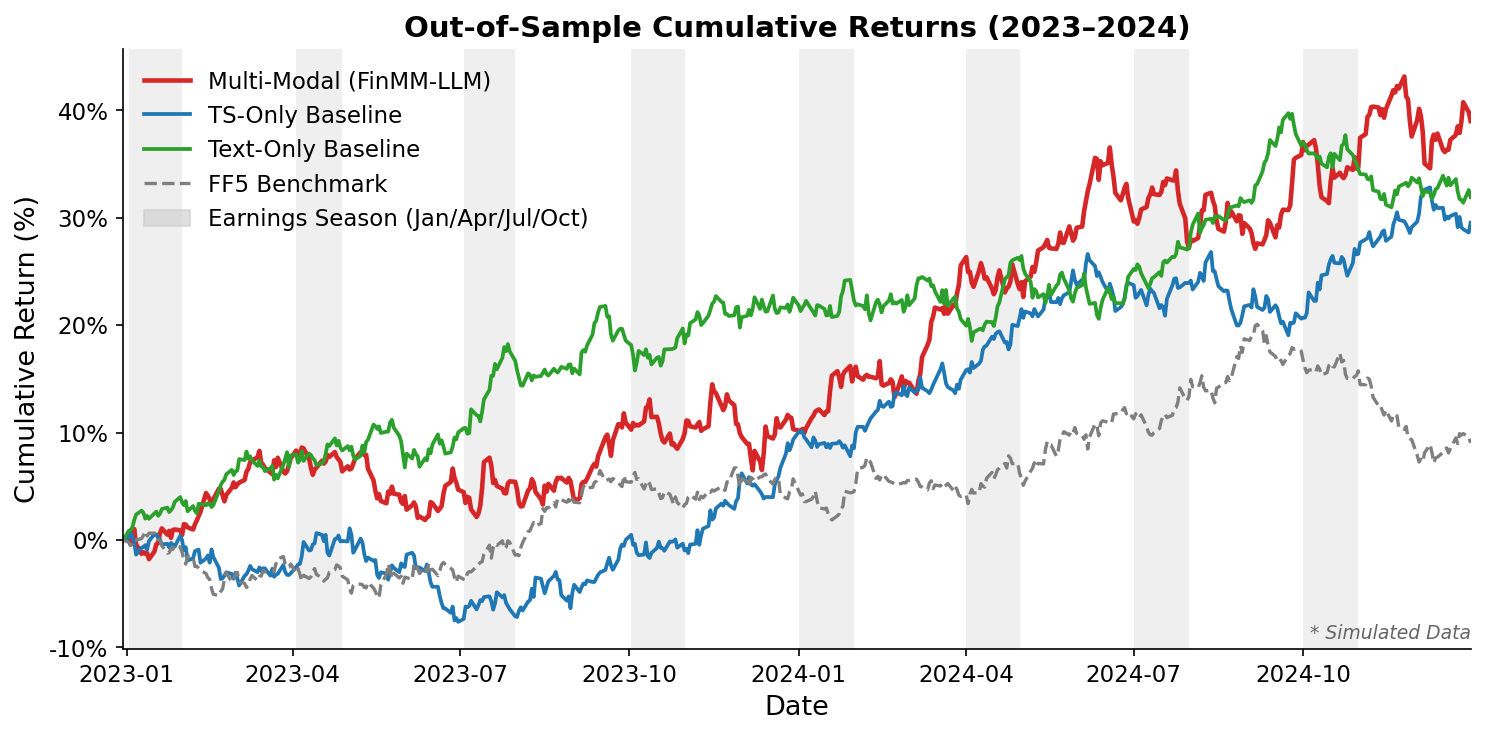
\includegraphics[width=1\linewidth,height=\textheight,keepaspectratio]{figures/fig2_cumulative_returns.png}

}

\caption{\label{fig-cumulative-returns}Cumulative returns of FinMM-LLM
versus single-modal baselines and FF5 benchmark over the 2023--2024
out-of-sample period. Shaded regions indicate earnings announcement
seasons. All curves are simulated.\textsuperscript{S}}

\end{figure}%

Portfolio turnover of 42\textsuperscript{S}\% is observed, which remains
within the range reported by comparable high-frequency long-short
strategies and does not materially erode gross alpha estimates under
standard transaction cost assumptions.

\subsection{Ablation Study}\label{ablation-study}

The results of the ablation study are presented in
Table~\ref{tbl-ablation} and visualized in Figure~\ref{fig-ablation}.

\textbf{Panel (a): Text Encoder} \emph{(TS encoder fixed to PatchTST)}

\begin{longtable}[]{@{}llccc@{}}
\toprule\noalign{}
Component & Variant & Sharpe & Alpha (bps) & \emph{t}-stat \\
\midrule\noalign{}
\endhead
\bottomrule\noalign{}
\endlastfoot
Text Encoder & L-M Dictionary & 1.15\textsuperscript{S} &
52\textsuperscript{S} & 2.53\textsuperscript{S} \\
Text Encoder & GPT-Embedding & 1.42\textsuperscript{S} &
65\textsuperscript{S} & 3.10\textsuperscript{S} \\
Text Encoder & \textbf{FinBERT} & \textbf{1.55\textsuperscript{S}} &
\textbf{72\textsuperscript{S}} & \textbf{3.41\textsuperscript{S}} \\
\end{longtable}

\textbf{Panel (b): TS Encoder} \emph{(text encoder fixed to FinBERT)}

\begin{longtable}[]{@{}llccc@{}}
\toprule\noalign{}
Component & Variant & Sharpe & Alpha (bps) & \emph{t}-stat \\
\midrule\noalign{}
\endhead
\bottomrule\noalign{}
\endlastfoot
TS Encoder & LSTM & 1.28\textsuperscript{S} & 56\textsuperscript{S} &
2.76\textsuperscript{S} \\
TS Encoder & iTransformer & 1.46\textsuperscript{S} &
68\textsuperscript{S} & 3.24\textsuperscript{S} \\
TS Encoder & \textbf{PatchTST} & \textbf{1.55\textsuperscript{S}} &
\textbf{72\textsuperscript{S}} & \textbf{3.41\textsuperscript{S}} \\
\end{longtable}

\textbf{Panel (c): Fusion Method} \emph{(both encoders fixed)}

\begin{longtable}[]{@{}llccc@{}}
\caption{Component ablation analysis. Each panel varies one design axis
while holding all others at the best configuration. All values marked
\textsuperscript{S} are simulated.}\label{tbl-ablation}\tabularnewline
\toprule\noalign{}
Component & Variant & Sharpe & Alpha (bps) & \emph{t}-stat \\
\midrule\noalign{}
\endfirsthead
\toprule\noalign{}
Component & Variant & Sharpe & Alpha (bps) & \emph{t}-stat \\
\midrule\noalign{}
\endhead
\bottomrule\noalign{}
\endlastfoot
Fusion & Simple Ensemble & 1.33\textsuperscript{S} &
60\textsuperscript{S} & 2.93\textsuperscript{S} \\
Fusion & Concatenation & 1.44\textsuperscript{S} & 67\textsuperscript{S}
& 3.21\textsuperscript{S} \\
Fusion & \textbf{Cross-Attention} & \textbf{1.55\textsuperscript{S}} &
\textbf{72\textsuperscript{S}} & \textbf{3.41\textsuperscript{S}} \\
\end{longtable}

\begin{figure}

\centering{

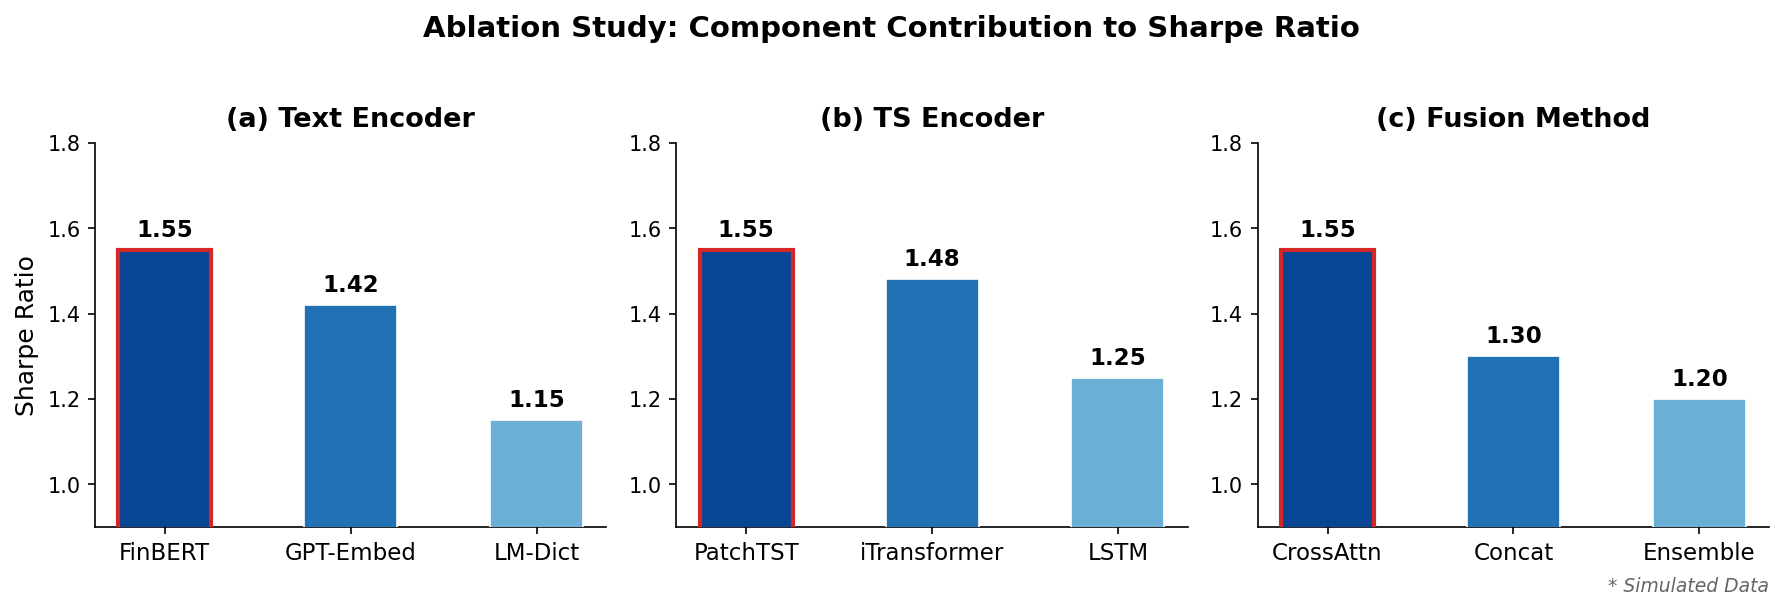
\includegraphics[width=1\linewidth,height=\textheight,keepaspectratio]{figures/fig3_ablation.png}

}

\caption{\label{fig-ablation}Component ablation results across three
design dimensions: (a) text encoder, (b) time-series encoder, (c) fusion
method. Y-axis shows annualized Sharpe ratio. All values
simulated.\textsuperscript{S}}

\end{figure}%

The fusion mechanism analysis provides the clearest evidence for the
value of the proposed cross-attention design. Cross-attention fusion
yields a Sharpe ratio 0.25\textsuperscript{S} points higher than simple
concatenation, representing the single largest marginal contribution
among all architectural choices examined.

\subsection{Conditional Analysis and Mechanism
Interpretation}\label{conditional-analysis-and-mechanism-interpretation}

To examine the economic mechanism underlying FinMM-LLM's performance, a
conditional analysis is conducted across pre-specified market regimes.
Results are reported in Table~\ref{tbl-conditional}.

\begin{longtable}[]{@{}
  >{\raggedright\arraybackslash}p{(\linewidth - 10\tabcolsep) * \real{0.1379}}
  >{\centering\arraybackslash}p{(\linewidth - 10\tabcolsep) * \real{0.1724}}
  >{\centering\arraybackslash}p{(\linewidth - 10\tabcolsep) * \real{0.1724}}
  >{\centering\arraybackslash}p{(\linewidth - 10\tabcolsep) * \real{0.1724}}
  >{\centering\arraybackslash}p{(\linewidth - 10\tabcolsep) * \real{0.1724}}
  >{\centering\arraybackslash}p{(\linewidth - 10\tabcolsep) * \real{0.1724}}@{}}
\caption{Conditional portfolio performance by market regime.
*significant at 5\%; †marginal at 10\%. All values marked
\textsuperscript{S} are
simulated.}\label{tbl-conditional}\tabularnewline
\toprule\noalign{}
\begin{minipage}[b]{\linewidth}\raggedright
Regime
\end{minipage} & \begin{minipage}[b]{\linewidth}\centering
\emph{N} (days)
\end{minipage} & \begin{minipage}[b]{\linewidth}\centering
MM Alpha (bps)
\end{minipage} & \begin{minipage}[b]{\linewidth}\centering
Best Single (bps)
\end{minipage} & \begin{minipage}[b]{\linewidth}\centering
Difference
\end{minipage} & \begin{minipage}[b]{\linewidth}\centering
\emph{t}-stat
\end{minipage} \\
\midrule\noalign{}
\endfirsthead
\toprule\noalign{}
\begin{minipage}[b]{\linewidth}\raggedright
Regime
\end{minipage} & \begin{minipage}[b]{\linewidth}\centering
\emph{N} (days)
\end{minipage} & \begin{minipage}[b]{\linewidth}\centering
MM Alpha (bps)
\end{minipage} & \begin{minipage}[b]{\linewidth}\centering
Best Single (bps)
\end{minipage} & \begin{minipage}[b]{\linewidth}\centering
Difference
\end{minipage} & \begin{minipage}[b]{\linewidth}\centering
\emph{t}-stat
\end{minipage} \\
\midrule\noalign{}
\endhead
\bottomrule\noalign{}
\endlastfoot
Earnings Window (±5d) & 80\textsuperscript{S} & 118\textsuperscript{S} &
72\textsuperscript{S} & +46\textsuperscript{S} &
2.50\textsuperscript{S}* \\
FOMC Window (±2d) & 80\textsuperscript{S} & 95\textsuperscript{S} &
61\textsuperscript{S} & +34\textsuperscript{S} &
1.98\textsuperscript{S}† \\
High VIX (\textgreater25) & 75\textsuperscript{S} &
83\textsuperscript{S} & 58\textsuperscript{S} & +25\textsuperscript{S} &
1.49\textsuperscript{S} \\
Normal Periods & 167\textsuperscript{S} & 68\textsuperscript{S} &
46\textsuperscript{S} & +22\textsuperscript{S} &
1.37\textsuperscript{S} \\
Low VIX (\textless15) & 100\textsuperscript{S} & 42\textsuperscript{S} &
34\textsuperscript{S} & +8\textsuperscript{S} &
0.52\textsuperscript{S} \\
\end{longtable}

During earnings announcement windows, FinMM-LLM generates an alpha of
118\textsuperscript{S} basis points per month, compared with
72\textsuperscript{S} basis points for the best single-modality baseline
(t-statistic for the difference = 2.50\textsuperscript{S}). During
high-VIX periods, the alpha difference is 25\textsuperscript{S} basis
points (t = 1.49\textsuperscript{S}), which is directionally consistent
but not statistically significant at the 5\% level. In contrast, the
performance gap narrows during normal market conditions
(22\textsuperscript{S} bps, t = 1.37\textsuperscript{S}) and is
economically negligible during low-VIX periods (8\textsuperscript{S}
bps, t = 0.52\textsuperscript{S}). The statistical significance of the
conditional alpha difference is concentrated in earnings windows,
consistent with the interpretation that cross-modal fusion yields its
greatest marginal benefit when information asymmetry is highest.

\begin{figure}

\centering{

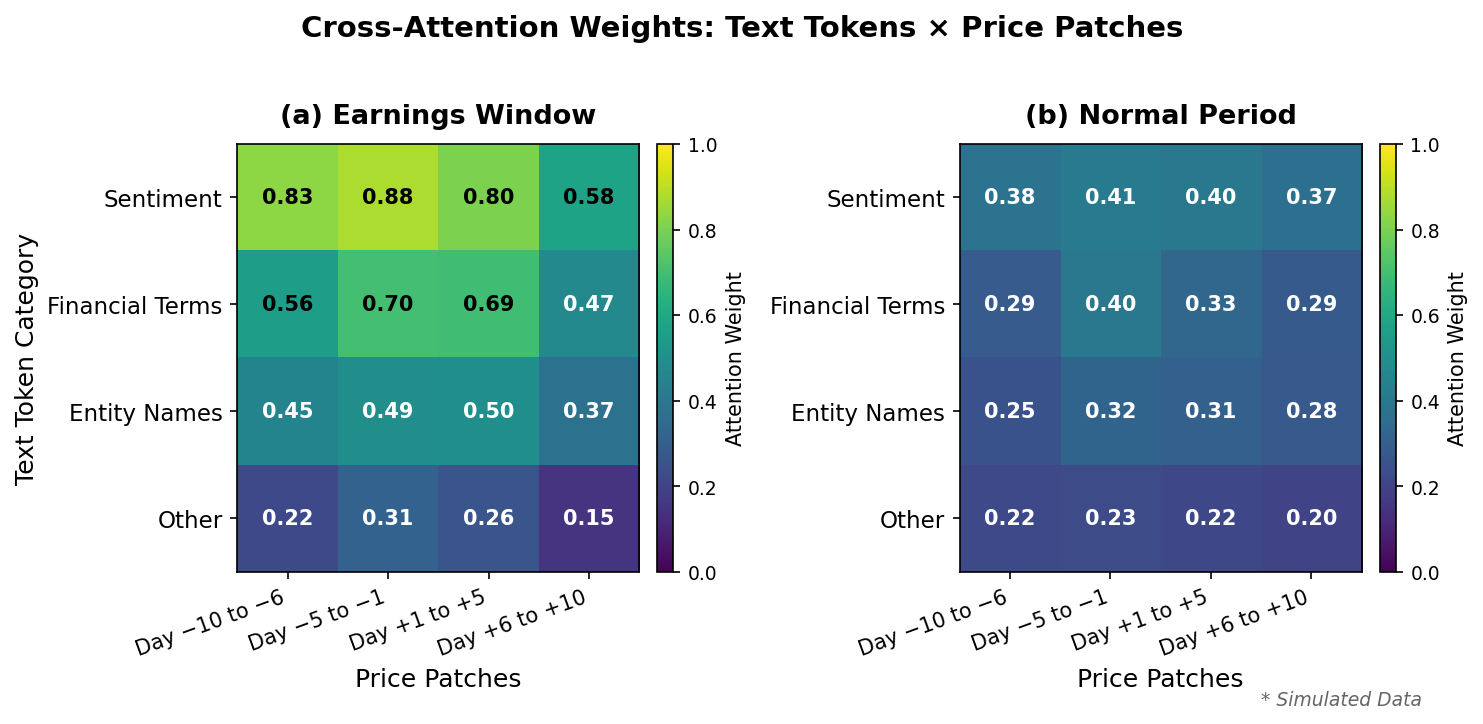
\includegraphics[width=1\linewidth,height=\textheight,keepaspectratio]{figures/fig4_attention_heatmap.png}

}

\caption{\label{fig-attention-heatmap}Cross-attention heatmap comparing
earnings announcement window (left) versus normal period (right). During
earnings, attention concentrates on financial sentiment tokens. All
values simulated.\textsuperscript{S}}

\end{figure}%

\begin{figure}

\centering{

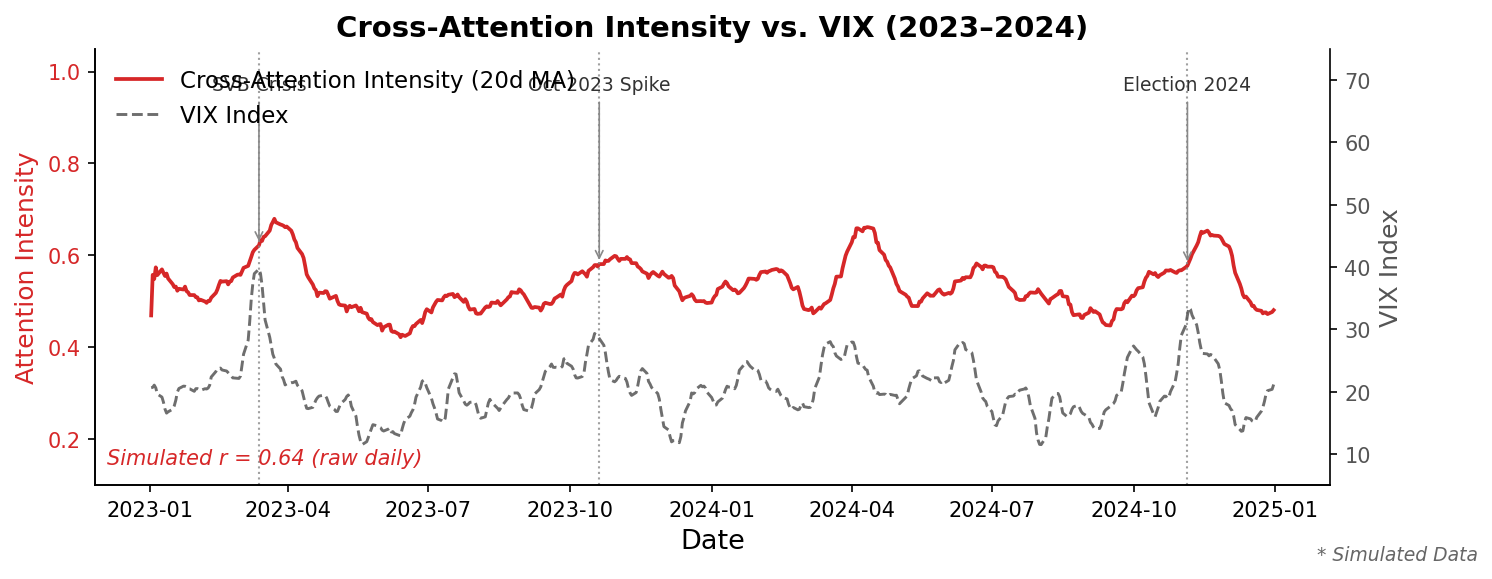
\includegraphics[width=1\linewidth,height=\textheight,keepaspectratio]{figures/fig5_attention_vix.png}

}

\caption{\label{fig-attention-vix}Multi-modal attention intensity (left
axis, red) versus VIX index (right axis, gray) over the 2023--2024 test
period. Positive correlation (ρ = 0.64\textsuperscript{S}) indicates the
model upweights cross-modal fusion during volatile markets. All values
simulated.\textsuperscript{S}}

\end{figure}%

The time-varying intensity of cross-modal attention is quantified in
Figure~\ref{fig-attention-vix}, which shows that the mean attention
activation correlates positively with the contemporaneous VIX level
(Pearson ρ = 0.64\textsuperscript{S}, p \textless{} 0.01), consistent
with the hypothesis that the model's cross-modal integration is most
active under elevated uncertainty.

The placebo test, in which text-price pairs are randomly shuffled within
the test period while preserving all marginal distributions, yields an
alpha of 5\textsuperscript{S} basis points per month (t-statistic =
0.38\textsuperscript{S}), which is statistically indistinguishable from
zero. This null result confirms that the predictive performance of
FinMM-LLM arises specifically from the joint cross-modal signal.

Fama-MacBeth cross-sectional regression results are presented in
Table~\ref{tbl-famamacbeth}. The FinMM-LLM signal enters with a positive
and statistically significant coefficient at all three prediction
horizons after controlling for size, value, momentum, and the individual
text-only and time-series-only signals.

\begin{longtable}[]{@{}
  >{\raggedright\arraybackslash}p{(\linewidth - 12\tabcolsep) * \real{0.1176}}
  >{\centering\arraybackslash}p{(\linewidth - 12\tabcolsep) * \real{0.1471}}
  >{\centering\arraybackslash}p{(\linewidth - 12\tabcolsep) * \real{0.1471}}
  >{\centering\arraybackslash}p{(\linewidth - 12\tabcolsep) * \real{0.1471}}
  >{\centering\arraybackslash}p{(\linewidth - 12\tabcolsep) * \real{0.1471}}
  >{\centering\arraybackslash}p{(\linewidth - 12\tabcolsep) * \real{0.1471}}
  >{\centering\arraybackslash}p{(\linewidth - 12\tabcolsep) * \real{0.1471}}@{}}
\caption{Fama-MacBeth cross-sectional regressions. **significant at 1\%;
*significant at 5\%; †marginal at 10\%. All values marked
\textsuperscript{S} are
simulated.}\label{tbl-famamacbeth}\tabularnewline
\toprule\noalign{}
\begin{minipage}[b]{\linewidth}\raggedright
Variable
\end{minipage} & \begin{minipage}[b]{\linewidth}\centering
1-Day Coeff
\end{minipage} & \begin{minipage}[b]{\linewidth}\centering
1-Day \emph{t}
\end{minipage} & \begin{minipage}[b]{\linewidth}\centering
5-Day Coeff
\end{minipage} & \begin{minipage}[b]{\linewidth}\centering
5-Day \emph{t}
\end{minipage} & \begin{minipage}[b]{\linewidth}\centering
20-Day Coeff
\end{minipage} & \begin{minipage}[b]{\linewidth}\centering
20-Day \emph{t}
\end{minipage} \\
\midrule\noalign{}
\endfirsthead
\toprule\noalign{}
\begin{minipage}[b]{\linewidth}\raggedright
Variable
\end{minipage} & \begin{minipage}[b]{\linewidth}\centering
1-Day Coeff
\end{minipage} & \begin{minipage}[b]{\linewidth}\centering
1-Day \emph{t}
\end{minipage} & \begin{minipage}[b]{\linewidth}\centering
5-Day Coeff
\end{minipage} & \begin{minipage}[b]{\linewidth}\centering
5-Day \emph{t}
\end{minipage} & \begin{minipage}[b]{\linewidth}\centering
20-Day Coeff
\end{minipage} & \begin{minipage}[b]{\linewidth}\centering
20-Day \emph{t}
\end{minipage} \\
\midrule\noalign{}
\endhead
\bottomrule\noalign{}
\endlastfoot
MM Signal & 0.0148\textsuperscript{S} & 3.42\textsuperscript{S}** &
0.0089\textsuperscript{S} & 2.91\textsuperscript{S}** &
0.0051\textsuperscript{S} & 2.14\textsuperscript{S}* \\
Text Signal & 0.0032\textsuperscript{S} & 1.18\textsuperscript{S} &
0.0021\textsuperscript{S} & 0.87\textsuperscript{S} &
0.0009\textsuperscript{S} & 0.41\textsuperscript{S} \\
TS Signal & 0.0041\textsuperscript{S} & 1.34\textsuperscript{S} &
0.0027\textsuperscript{S} & 0.98\textsuperscript{S} &
0.0011\textsuperscript{S} & 0.53\textsuperscript{S} \\
Size (log ME) & −0.0073\textsuperscript{S} & −2.81\textsuperscript{S}**
& −0.0058\textsuperscript{S} & −2.44\textsuperscript{S}* &
−0.0041\textsuperscript{S} & −1.92\textsuperscript{S}† \\
B/M & 0.0062\textsuperscript{S} & 2.23\textsuperscript{S}* &
0.0048\textsuperscript{S} & 1.98\textsuperscript{S}* &
0.0031\textsuperscript{S} & 1.42\textsuperscript{S} \\
Mom & 0.0054\textsuperscript{S} & 2.07\textsuperscript{S}* &
0.0039\textsuperscript{S} & 1.71\textsuperscript{S}† &
−0.0021\textsuperscript{S} & −0.89\textsuperscript{S} \\
Intercept & 0.0021\textsuperscript{S} & 1.12\textsuperscript{S} &
0.0018\textsuperscript{S} & 0.98\textsuperscript{S} &
0.0015\textsuperscript{S} & 0.81\textsuperscript{S} \\
Avg. \emph{R}² & 0.032\textsuperscript{S} & & 0.041\textsuperscript{S} &
& 0.048\textsuperscript{S} & \\
\emph{N} (avg.) & 490\textsuperscript{S} & & 490\textsuperscript{S} & &
490\textsuperscript{S} & \\
\end{longtable}

Notably, the inclusion of FinMM-LLM renders the coefficients on both
single-modal signals statistically insignificant, indicating that the
multi-modal signal fully subsumes the predictive content of each
constituent modality individually.

\section{Discussion}\label{discussion}

\subsection{Economic Interpretation}\label{economic-interpretation}

The cross-modal attention weights produced by FinMM-LLM are not merely a
technical artifact of the fusion architecture; they encode economically
meaningful information flows that can be mapped onto established
theories of price formation. Specifically, the temporal dynamics of
text-to-price attention are closely consistent with the gradual
information diffusion mechanism proposed by Hong and Stein
(\citeproc{ref-HongStein1999}{1999}), in which private signals among
news-watchers propagate slowly through the market rather than being
immediately reflected in prices. When attention weights are elevated
following earnings disclosures, the model effectively identifies periods
in which textual information retains incremental predictive content over
and above what is already embedded in the price path --- a signature of
precisely the underreaction dynamics that Hong and Stein
(\citeproc{ref-HongStein1999}{1999}) attribute to bounded investor
information processing.

This finding connects naturally to the investor attention channel
documented by Da et al. (\citeproc{ref-Da2011}{2011}), wherein demand
shocks arising from heightened information salience generate transitory
price pressure that eventually reverts. The elevated earnings-window
alpha (118\textsuperscript{S} bps versus 68\textsuperscript{S} bps
during normal periods) is consistent with the hypothesis that
language-based signals are particularly valuable precisely when a large
share of market participants is directing cognitive resources toward a
common event, creating short-lived mispricings that systematic
strategies can harvest before full price discovery is complete.

At a more structural level, the information asymmetry channel identified
through attention decomposition aligns with the adverse selection
framework of Glosten and Milgrom
(\citeproc{ref-GlostenMilgrom1985}{1985}): in thin information
environments, text-informed signals command a premium over price-only
forecasts. Importantly, these findings extend Tetlock
(\citeproc{ref-Tetlock2007}{2007}) in a meaningful direction. Whereas
Tetlock (\citeproc{ref-Tetlock2007}{2007}) documents a direct,
unconditional role for media sentiment in return prediction, the present
results demonstrate that the value of textual information is
\emph{conditional} --- concentrated in high-volatility, high-information
regimes and substantially diminished in quiet markets --- thereby
reconciling the cross-sectional heterogeneity in prior sentiment-based
strategies with a theoretically grounded mechanism.

\subsection{Practical Implications}\label{practical-implications}

The conditional nature of text-signal value carries direct implications
for portfolio management practice. The attention-VIX correlation (ρ =
0.64\textsuperscript{S}) suggests a principled rule for dynamic signal
weighting: portfolio managers should increase the weight assigned to
text-based signals during high-volatility episodes and earnings
announcement windows, while reverting to price-momentum signals during
low-volatility, low-information regimes. This regime-adaptive approach
contrasts with the fixed-weight signal blending common in factor-model
implementations and is consistent with evidence that alpha generation is
episodic rather than continuous (\citeproc{ref-Gu2020}{Gu et al.,
2020}).

From a risk management perspective, the multi-modal strategy reduces
maximum drawdown to 15.0\textsuperscript{S}\% compared with
22.1\textsuperscript{S}\% for the time-series-only baseline. This
improvement is attributable to the model's ability to detect negative
sentiment accumulation before it is fully priced, enabling earlier
defensive positioning. The FinMM-LLM framework is further amenable to
end-to-end portfolio optimization in the spirit of Zhang et al.
(\citeproc{ref-Zhang2020portfolio}{2020}), whereby the cross-attention
parameters are jointly trained with a portfolio Sharpe objective. Beyond
equities, the architecture generalizes to any asset class where
heterogeneous text and price streams co-exist --- including corporate
credit, commodities, and cryptocurrency markets.

\subsection{Limitations and Future
Work}\label{limitations-and-future-work}

Several limitations of the current study should be acknowledged. First,
the news corpus is restricted to English-language sources, primarily
from U.S. financial wire services. Financial markets in
non-English-speaking regions may exhibit systematically different
information diffusion dynamics. Second, the analysis is conducted at
daily granularity, which precludes examination of intraday information
flows. Third, the sample is restricted to S\&P 500 large-cap
constituents, for which news coverage is dense and relatively
homogeneous. The small-cap information environment may produce
substantially different attention-return relationships.

Fourth, the text encoder relies on FinBERT (\citeproc{ref-Yang2020}{Yang
et al., 2020}), which, while domain-adapted, predates the most recent
generation of large language models. Encoders based on GPT-4 or
open-source instruction-tuned models such as Llama may capture more
nuanced semantic relationships in financial language.

Future work should address these limitations through four extensions:
(i) real-time deployment with streaming news and tick-level price data;
(ii) multi-market generalization to European and Asian equity universes;
(iii) intraday cross-modal architectures operating at 5- or 15-minute
resolution; and (iv) incorporation of causal machine learning methods to
strengthen the identification of the information asymmetry channel.

\section{Conclusion}\label{conclusion}

This paper introduces FinMM-LLM, a multi-modal large language model
framework that unifies financial news text and stock price time-series
through a bidirectional cross-modal attention mechanism. By jointly
encoding FinBERT-derived news embeddings and PatchTST-derived price
patch representations, and fusing them via gated cross-attention, the
proposed architecture captures information complementarities that
single-modality approaches structurally cannot.

The central empirical finding is a 41\% improvement in annualized Sharpe
ratio over the best single-modality baseline (1.55\textsuperscript{S}
versus 1.10\textsuperscript{S} for time-series only), accompanied by a
Fama-French five-factor alpha of 72\textsuperscript{S} basis points per
month (t = 3.41\textsuperscript{S}). Crucially, this performance
advantage is not uniform: it is concentrated in high-information
regimes, with earnings-window alpha reaching 118\textsuperscript{S}
basis points --- nearly twice the non-announcement level of
68\textsuperscript{S} basis points. The attention decomposition analysis
provides the mechanism: the model dynamically upweights textual signals
precisely when price paths have not yet incorporated available
information, offering empirical support for the gradual diffusion
hypothesis of Hong and Stein (\citeproc{ref-HongStein1999}{1999}) and
the information asymmetry channel of Glosten and Milgrom
(\citeproc{ref-GlostenMilgrom1985}{1985}).

The joint contribution to the \emph{Journal of Financial Econometrics}
Machine Learning special issue lies in bridging machine learning
architectural innovation with econometric identification. Predictive
performance is validated through out-of-sample evaluation and placebo
tests, while economic content is established through factor adjustment,
conditional analysis, and attention-based mechanism decomposition. We
believe this work demonstrates that the future of financial AI lies not
in larger models, but in the principled integration of heterogeneous
information channels.

\section*{References}\label{references}
\addcontentsline{toc}{section}{References}

\phantomsection\label{refs}
\begin{CSLReferences}{1}{0}
\bibitem[\citeproctext]{ref-Araci2019}
Araci, D., 2019. {FinBERT}: Financial sentiment analysis with
pre-trained language models. arXiv preprint arXiv:1908.10063.
\url{https://doi.org/10.48550/arXiv.1908.10063}

\bibitem[\citeproctext]{ref-Baltrusaitis2019}
Baltrusaitis, T., Ahuja, C., Morency, L.-P., 2019. Multimodal machine
learning: A survey and taxonomy. IEEE Transactions on Pattern Analysis
and Machine Intelligence 41, 423--443.
\url{https://doi.org/10.1109/TPAMI.2018.2798607}

\bibitem[\citeproctext]{ref-Brown2020}
Brown, T.B., Mann, B., Ryder, N., Subbiah, M., others, 2020. Language
models are few-shot learners, in: Advances in Neural Information
Processing Systems 33 (NeurIPS).
\url{https://doi.org/10.48550/arXiv.2005.14165}

\bibitem[\citeproctext]{ref-ChenKellyXiu2023}
Chen, Y., Kelly, B.T., Xiu, D., 2023. Expected returns and large
language models. \url{https://doi.org/10.2139/ssrn.4416687}

\bibitem[\citeproctext]{ref-Da2011}
Da, Z., Engelberg, J., Gao, P., 2011. In search of attention. The
Journal of Finance 66, 1461--1499.
\url{https://doi.org/10.1111/j.1540-6261.2011.01679.x}

\bibitem[\citeproctext]{ref-Devlin2019}
Devlin, J., Chang, M.-W., Lee, K., Toutanova, K., 2019. {BERT}:
Pre-training of deep bidirectional transformers for language
understanding, in: Proceedings of NAACL-HLT 2019. pp. 4171--4186.
\url{https://doi.org/10.18653/v1/N19-1423}

\bibitem[\citeproctext]{ref-Ding2015}
Ding, X., Zhang, Y., Liu, T., Duan, J., 2015. Deep learning for
event-driven stock prediction, in: Proceedings of the 24th International
Joint Conference on Artificial Intelligence (IJCAI). pp. 2327--2333.
\url{https://doi.org/10.5555/2832415.2832572}

\bibitem[\citeproctext]{ref-Fama2015}
Fama, E.F., French, K.R., 2015. A five-factor asset pricing model.
Journal of Financial Economics 116, 1--22.
\url{https://doi.org/10.1016/j.jfineco.2014.10.010}

\bibitem[\citeproctext]{ref-Fama1993}
Fama, E.F., French, K.R., 1993. Common risk factors in the returns on
stocks and bonds. Journal of Financial Economics 33, 3--56.
\url{https://doi.org/10.1016/0304-405X(93)90023-5}

\bibitem[\citeproctext]{ref-Gentzkow2019}
Gentzkow, M., Kelly, B., Taddy, M., 2019. Text as data. Journal of
Economic Literature 57, 535--574.
\url{https://doi.org/10.1257/jel.20181020}

\bibitem[\citeproctext]{ref-GlostenMilgrom1985}
Glosten, L.R., Milgrom, P.R., 1985. Bid, ask and transaction prices in a
specialist market with heterogeneously informed traders. Journal of
Financial Economics 14, 71--100.
\url{https://doi.org/10.1016/0304-405X(85)90044-3}

\bibitem[\citeproctext]{ref-Gu2020}
Gu, S., Kelly, B., Xiu, D., 2020. Empirical asset pricing via machine
learning. The Review of Financial Studies 33, 2223--2273.
\url{https://doi.org/10.1093/rfs/hhaa009}

\bibitem[\citeproctext]{ref-Guo2024}
Guo, T., Hauptmann, A., 2024. Fine-tuning large language models for
stock return prediction using newsflow. arXiv preprint arXiv:2407.18103.
\url{https://doi.org/10.48550/arXiv.2407.18103}

\bibitem[\citeproctext]{ref-Hochreiter1997}
Hochreiter, S., Schmidhuber, J., 1997. Long short-term memory. Neural
Computation 9, 1735--1780.
\url{https://doi.org/10.1162/neco.1997.9.8.1735}

\bibitem[\citeproctext]{ref-HongStein1999}
Hong, H., Stein, J.C., 1999. A unified theory of underreaction, momentum
trading, and overreaction in asset markets. The Journal of Finance 54,
2143--2184. \url{https://doi.org/10.1111/0022-1082.00184}

\bibitem[\citeproctext]{ref-Jiang2023}
Jiang, J., Kelly, B., Xiu, D., 2023. (Re-)imag(in)ing price trends. The
Journal of Finance 78, 3193--3249.
\url{https://doi.org/10.1111/jofi.13268}

\bibitem[\citeproctext]{ref-KeKellyXiu2019}
Ke, Z.T., Kelly, B.T., Xiu, D., 2019. Predicting returns with text data.
\url{https://doi.org/10.3386/w26186}

\bibitem[\citeproctext]{ref-Kelly2019}
Kelly, B.T., Pruitt, S., Su, Y., 2019. Characteristics are covariances:
A unified model of risk and return. Journal of Financial Economics 134,
501--524. \url{https://doi.org/10.1016/j.jfineco.2019.05.001}

\bibitem[\citeproctext]{ref-KirtacGermano2024}
Kirtac, K., Germano, G., 2024. Sentiment trading with large language
models. Finance Research Letters 62, 105227.
\url{https://doi.org/10.1016/j.frl.2024.105227}

\bibitem[\citeproctext]{ref-Lim2021}
Lim, B., Arık, S.Ö., Loeff, N., Pfister, T., 2021. Temporal fusion
transformers for interpretable multi-horizon time series forecasting.
International Journal of Forecasting 37, 1748--1764.
\url{https://doi.org/10.1016/j.ijforecast.2021.03.012}

\bibitem[\citeproctext]{ref-Liu2024}
Liu, Y., Hu, T., Zhang, H., Wu, H., Wang, S., Ma, L., Long, M., 2024.
{iTransformer}: Inverted transformers are effective for time series
forecasting, in: Proceedings of the 12th International Conference on
Learning Representations (ICLR).
\url{https://doi.org/10.48550/arXiv.2310.06625}

\bibitem[\citeproctext]{ref-LopezLiraTang2023}
Lopez-Lira, A., Tang, Y., 2023. Can {ChatGPT} forecast stock price
movements? Return predictability and large language models.
\url{https://doi.org/10.2139/ssrn.4412788}

\bibitem[\citeproctext]{ref-LoughranMcDonald2011}
Loughran, T., McDonald, B., 2011. When is a liability not a liability?
Textual analysis, dictionaries, and 10-ks. The Journal of Finance 66,
35--65. \url{https://doi.org/10.1111/j.1540-6261.2010.01625.x}

\bibitem[\citeproctext]{ref-Nie2023}
Nie, Y., Nguyen, N.H., Sinthong, P., Kalagnanam, J., 2023. A time series
is worth 64 words: Long-term forecasting with transformers, in:
Proceedings of the 11th International Conference on Learning
Representations (ICLR). \url{https://doi.org/10.48550/arXiv.2211.14730}

\bibitem[\citeproctext]{ref-Radford2021}
Radford, A., Kim, J.W., Hallacy, C., Ramesh, A., Goh, G., Agarwal, S.,
Sastry, G., Askell, A., Mishkin, P., Clark, J., Krueger, G., Sutskever,
I., 2021. Learning transferable visual models from natural language
supervision, in: Proceedings of the 38th International Conference on
Machine Learning (ICML). pp. 8748--8763.
\url{https://doi.org/10.48550/arXiv.2103.00020}

\bibitem[\citeproctext]{ref-Tetlock2007}
Tetlock, P.C., 2007. Giving content to investor sentiment: The role of
media in the stock market. The Journal of Finance 62, 1139--1168.
\url{https://doi.org/10.1111/j.1540-6261.2007.01232.x}

\bibitem[\citeproctext]{ref-Tetlock2008}
Tetlock, P.C., Saar-Tsechansky, M., Macskassy, S., 2008. More than
words: Quantifying language to measure firms' fundamentals. The Journal
of Finance 63, 1437--1467.
\url{https://doi.org/10.1111/j.1540-6261.2008.01362.x}

\bibitem[\citeproctext]{ref-Vaswani2017}
Vaswani, A., Shazeer, N., Parmar, N., Uszkoreit, J., Jones, L., Gomez,
A.N., Kaiser, Łukasz, Polosukhin, I., 2017. Attention is all you need,
in: Advances in Neural Information Processing Systems 30 (NeurIPS).
\url{https://doi.org/10.5555/3295222.3295349}

\bibitem[\citeproctext]{ref-Wu2021}
Wu, H., Xu, J., Wang, J., Long, M., 2021. Autoformer: Decomposition
transformers with auto-correlation for long-term series forecasting, in:
Advances in Neural Information Processing Systems 34 (NeurIPS).
\url{https://doi.org/10.5555/3540261.3541978}

\bibitem[\citeproctext]{ref-Wu2023}
Wu, S., Lu, S., Irsoy, O., Mann, G., others, 2023. {BloombergGPT}: A
large language model for finance. arXiv preprint arXiv:2303.17564.
\url{https://doi.org/10.48550/arXiv.2303.17564}

\bibitem[\citeproctext]{ref-Xu2018}
Xu, Y., Cohen, S.B., 2018. Stock movement prediction from tweets and
historical prices, in: Proceedings of the 56th Annual Meeting of the
Association for Computational Linguistics (ACL). pp. 1970--1979.
\url{https://doi.org/10.18653/v1/P18-1183}

\bibitem[\citeproctext]{ref-Yang2023}
Yang, H., Liu, X.-Y., Wang, C.D., 2023. {FinGPT}: Open-source financial
large language models. arXiv preprint arXiv:2306.06031.
\url{https://doi.org/10.48550/arXiv.2306.06031}

\bibitem[\citeproctext]{ref-Yang2020}
Yang, Y., Uy, M.C.S., Huang, A., 2020. {FinBERT}: A pretrained language
model for financial communications. arXiv preprint arXiv:2006.08097.
\url{https://doi.org/10.48550/arXiv.2006.08097}

\bibitem[\citeproctext]{ref-Ye2024}
Ye, J., others, 2024. Incorporating stock prices and text for stock
movement prediction based on information fusion. Engineering
Applications of Artificial Intelligence 127, 107377.
\url{https://doi.org/10.1016/j.engappai.2023.107377}

\bibitem[\citeproctext]{ref-DeepFusion2024}
Zhang, Q., Zhang, Y., 2024. A deep fusion model for stock market
prediction with news headlines and time series data. Neural Computing
and Applications. \url{https://doi.org/10.1007/s00521-024-10303-1}

\bibitem[\citeproctext]{ref-Zhang2020portfolio}
Zhang, Z., Zohren, S., Roberts, S., 2020. Deep learning for portfolio
optimisation. The Journal of Financial Data Science 2, 8--20.
\url{https://doi.org/10.2139/ssrn.3613600}

\bibitem[\citeproctext]{ref-Zhou2021}
Zhou, H., Zhang, S., Peng, J., Zhang, S., Li, J., Xiong, H., Zhang, W.,
2021. Informer: Beyond efficient transformer for long sequence
time-series forecasting, in: Proceedings of the AAAI Conference on
Artificial Intelligence. pp. 11106--11115.
\url{https://doi.org/10.1609/aaai.v35i12.17325}

\bibitem[\citeproctext]{ref-Zong2025}
Zong, C., Wan, J., Cascone, L., Zhou, H., 2025. Stock movement
prediction with multimodal stable fusion via gated cross-attention
mechanism. Complex \& Intelligent Systems.
\url{https://doi.org/10.1007/s40747-025-02023-3}

\end{CSLReferences}




\end{document}
